\documentclass{article}
\usepackage[utf8]{inputenc}
\usepackage{graphicx}
\usepackage{float}

\title{
    \vspace{-4ex}
    Userguide for the authi-sign Extension
    \vspace{-4ex}
    }
\date{}
\begin{document}

\maketitle

\section{Login}
To use the extension and publish comments you first have to connect the extension with your ORCID iD and get the certificate:

\begin{enumerate}
    \item Click on the extension icon in the top right corner of the browser and select the \textit{authi-sign} extension.
        \begin{figure}[H]
            \centering
            \fbox{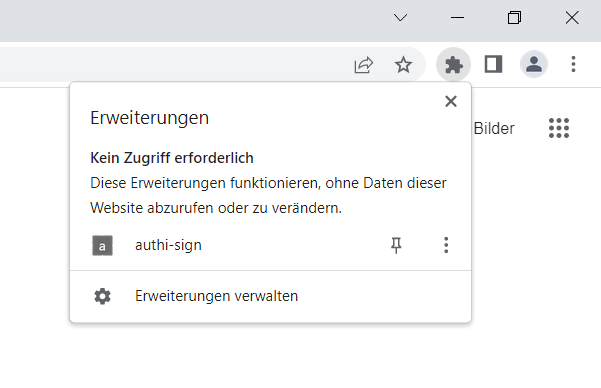
\includegraphics[scale=0.4]{01.png}}
        \end{figure}
    \item In the opened widget select the "Connect your ORCID iD" button. A new tab will open.
    \item In this tab select the button "Connect your ORCID iD" in your browser window. This will forward you to orcid.org.
    \item On the Orcid site enter your credentials for Orcid. You have to enter your password and either your ORCID iD or the e-mail address, that you are registered under on Orcid. Alternatively, you can also log into Orcid with your institutional access, your Google account or your Facebook account.
        \begin{figure}[H]
            \centering
            \fbox{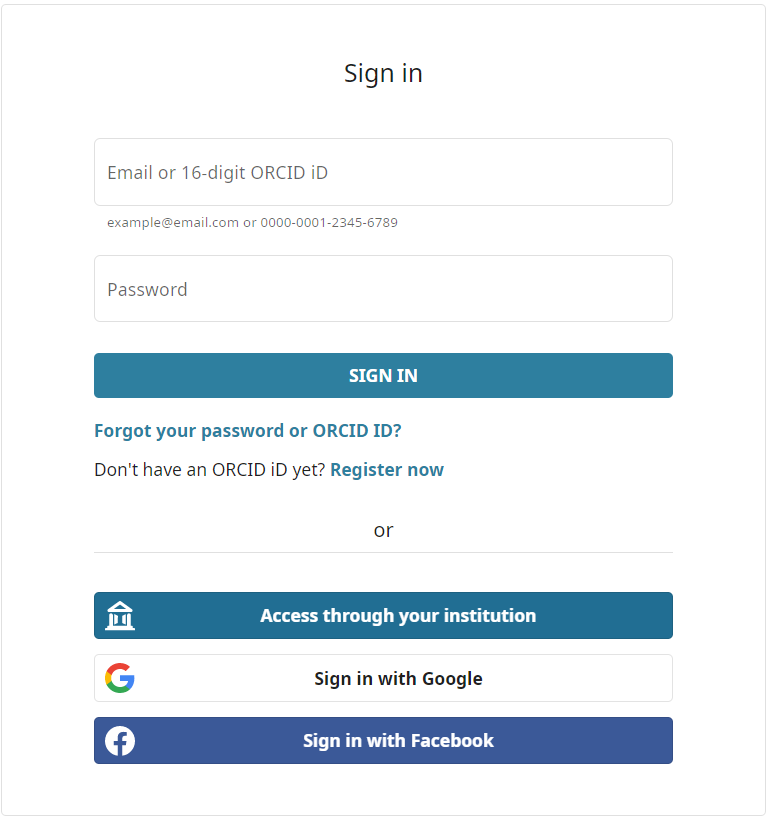
\includegraphics[scale=0.25]{02.png}}
        \end{figure}
    \item After successfully logging into your Orcid account a confirmation message will appear in the tab.
    \item To get the certificate, open the extension once again. Choose a name. This name will appear as the name of the author of the comments you publish. You can also enter your email address to have it stored inside the certificate as well.
    \item Lastly, click on "Get your certificate" and you are done!
\end{enumerate}

\section{General Overview}

\begin{figure}[H]
    \centering
    \fbox{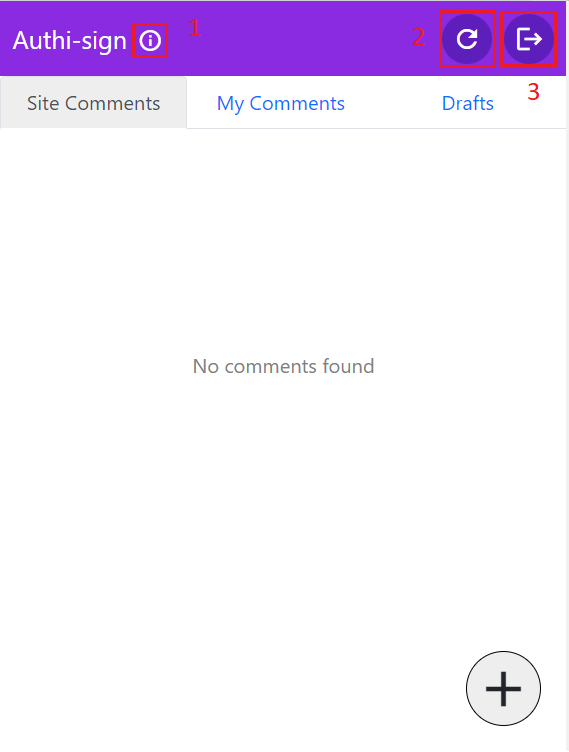
\includegraphics[scale=0.5]{03.png}}
\end{figure}

In the header of the extension there are three buttons: 
\begin{enumerate}
    \item The info button will open a new tab. In this tab you can see the imprint and information about the DSGVO compliance of the extension.
    \item The refresh button reloads the comments in the extension.
    \item The logout button logs you out of your current account. After logging out you will have to repeat the login process before you can use the extension again.\\\\\\\\\\\\\\
\end{enumerate}
Under the header you can select to view one of three different sections:
\begin{itemize}
    \item \textbf{Site Comments:} This section lists every comment from every user, but only for the site you are currently on.
    \item \textbf{My Comments:} Here you can see only your own comments that you published across every website.
        \begin{itemize}
            \item By clicking on any comment in the \textit{Site Comments} or the \textit{My Comments} section you can open an additional tab displaying further information about the comment.
        \end{itemize}
    \item \textbf{Drafts:} In this section are all the comments that you didn't publish, but instead chose to save as a draft.
    \begin{itemize}
        \item You can delete any drafts that you have saved here by clicking the \textit{Delete} button at the right side of every draft comment and confirming the action. This action can not be reversed. Any draft comments that are deleted this way are not retrievable.
    \end{itemize}
\end{itemize}

\section{Making Comments}
To start writing a new comment you first have to select the \textbf{+} button in the bottom right corner of the extension. This will open a new tab with the following contents:
\begin{figure}[H]
    \centering
    \fbox{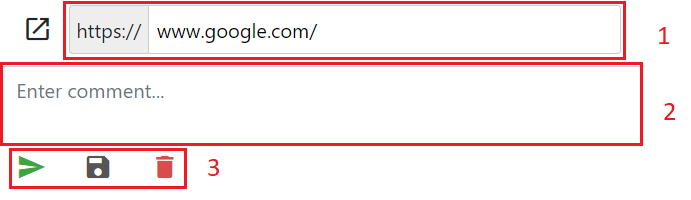
\includegraphics[scale=0.5]{04.png}}
\end{figure}

\begin{enumerate}
    \item Enter the website address to which you want to publish the comment to. The extension fills it in automatically with the website address you opened this tab from, but you can change it to any valid website address you want.
    \item Write the text for the comment.
    \item You can publish your comment by selecting the green \textit{Submit} button. Alternatively you can just save the comment as a draft by selecting the grey \textit{Save} button or you can delete your comment by selecting the red \textit{Delete} button.
\end{enumerate}

\end{document}
